\chapter{Questao 2}

\subsection*{Código}

\begin{python}
import pandas as pd
import numpy as np
import matplotlib.pyplot as plt

# pré convertido para utf-8
df = pd.read_csv('VIS_Pr_01_Vendas.csv')

df['order_year'] = pd.to_datetime(df['Order Date']).dt.strftime('%Y')

df = df.groupby(['Sub-Category','order_year']).agg(
    {'Profit': ['sum']}
).reset_index()

df.columns = [
    "_".join(t).strip('_').replace('-','_').lower()
    for t in df.columns
]

df = df.pivot(
    index='sub_category',
    columns='order_year',
    values=['profit_sum']
).reset_index()

df.columns = [
    (t[1] if ('profit_sum' in t) else t[0])
    for t in df.columns
]

sub_category = df['sub_category'].to_list()
values = df.drop('sub_category', axis=1).to_dict('list')


x = np.arange(len(sub_category))
width = 0.15
multiplier = 0

fig, ax = plt.subplots(
    constrained_layout=True,
    figsize=(15, 7)
)

for attribute, measurement in values.items():
    
    rgb = (
        (12*(5**(-multiplier))*(10**multiplier))/255,
        (34+(45*multiplier))/255,
        (150+(30*multiplier))/255,
    )    
    
    offset = width * multiplier
    rects = ax.bar(
        x + offset,
        measurement,
        width,
        label=attribute,
        color=rgb)
        
    multiplier += 1

ax.set_ylabel('profit')
ax.set_xticks(x + width, sub_category)
ax.legend(loc='upper left')
ax.grid(axis = 'y')

plt.show()'
\end{python}


\subsection*{plot}
\begin{figure}[h]
	\centering
	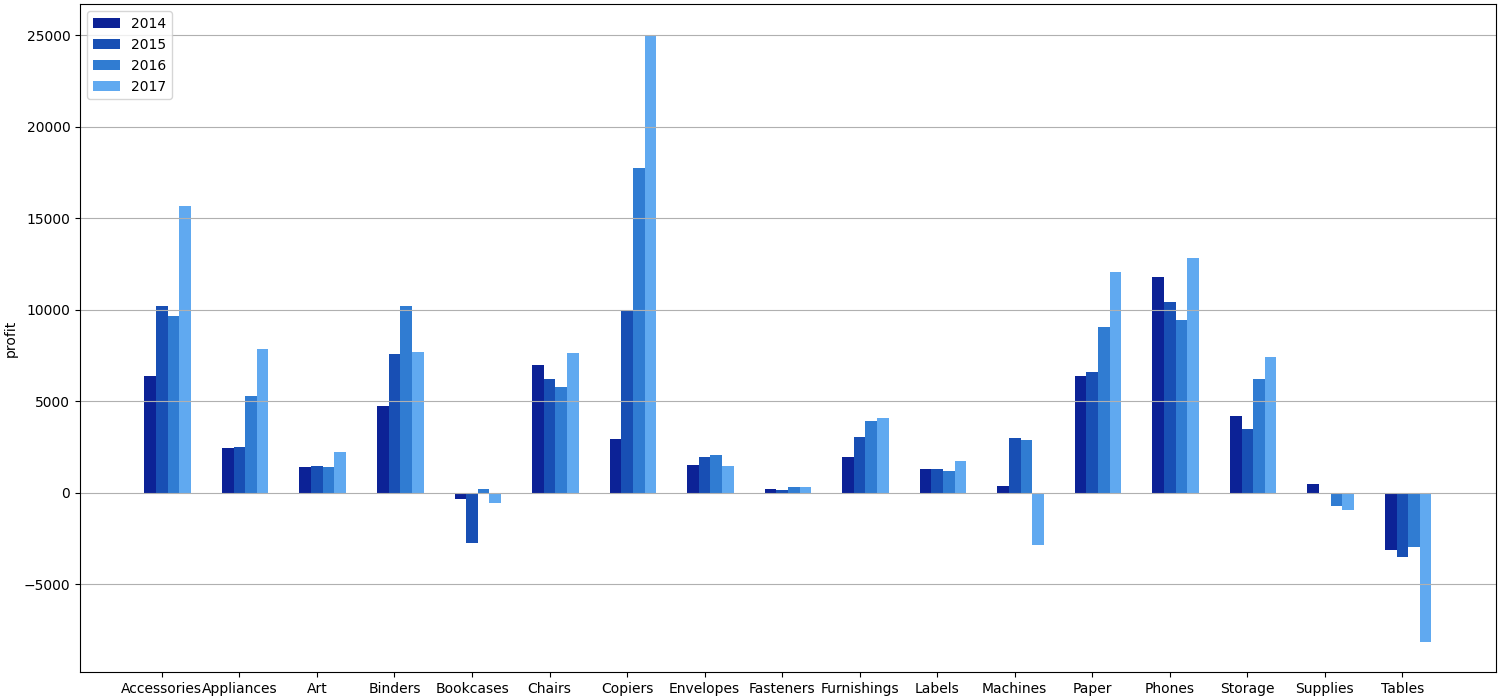
\includegraphics[width=\textwidth,keepaspectratio]{figures/graph_bar}
	\caption{diagrama do modelo - dedução da matriz}
	\label{lof}
\end{figure}

\subsection*{Comentários}
Os gráficos do matplotlib embora podem ser facilmente personalizados,
exigem um código mais extenso para o caso de houver mais dados e quiser manter a personalização de esquemas de cores do gráfico.